%!TEX root = Thesis.tex

\chapter{Clustering}
\label{chapter:clustering}

\section{The problem of clustering}
\label{sec:clustering}

% have to say that I'm using a vectorial representation of the data (data as vector of features) without loss of generality. I have to specify that I'm dealing with a partitioning clustering but other kinds exist. In this context (of vectorial data and partitional algorithms) K-Means is one of the most known algorithms. It's simple and fast and, although it only yields good results in a specific set of cases, it's often used as a starting point for more robust algorithms, e.g. EAC. 

%this is mostly taken from Jain's 50 years beyond K-Means
Hundreds of methods for data analysis exist.
Many of these methods fall into the realm of machine learning, which is usually divided into 2 major groups: \textit{supervised} and \textit{unsupervised} learning.
% TODO: add some reference for the 2 major groups; optional: explain what learning is
Supervised learning deals with labeled data, i.e. data for which ground truth is known, and tries to solve the problem of classification.
Examples of supervised learning algorithms are Neural Networks, Decision Trees, Linear Regression and Support Vector Machines. %TODO add refs
 %TODO: add ref for solving classification
Unsupervised learning deals with unlabeled data for which no extra information is known.
Clustering algorithms, expectation-maximization and Principal Component Analysis are examples of unsupervised algorithms. % TODO: add refs

Cluster analysis methods are unsupervised and the backbone of the present work.
The goal of data clustering, as defined by \cite{Jain2010}, is the discovery of the \textit{natural grouping(s)} of a set of patterns, points or objects.
In other words, the goal of data clustering is to discover structure on data.
The methodology used is to group patterns (usually represented as a vector of measurements or a point in space \cite{Jain1999}) based on some similarity, such that patterns belonging to the same cluster are typically more similar to each other than to patterns of other clusters.
Clustering is a strictly data-driven method, in contrast with classification techniques which have a training set with the desired labels for a limited collection of patterns.
Because there is very little information, as few assumptions as possible should be made about the structure of the data (e.g. number of clusters).
And, because clustering typically makes as few assumptions on the data as possible, it is appropriate to use it on exploratory structural analysis of the data.
The process of clustering data has three main stages \cite{Jain1999}:

\begin{itemize}
    \item \textbf{Pattern representation} refers to the choice of representation of the input data in terms of size, scale and type of features.
    The input patterns may be fed directly to the algorithms or undergo \emph{feature selection} and/or \emph{feature extraction}. The former is simply the selection of which features of the originally available should be used.
    The later deals with the transformation of the original features such that the resulting features will produce more accurate and insightful clusterings, e.g. Principal Component Analysis.
    % It should be noted that

    \item \textbf{Pattern similarity} refers to the definition of a measure for computing the similarity between two patterns.
    \item \textbf{Grouping} refers to the algorithm that will perform the actual clustering on the dataset with the defined pattern representation, using the appropriate similarity measure.
\end{itemize}

As an example, Figure \ref{fig:intro raw} shows the plot of the Iris data set, a small benchmark Machine Learning data set.
This data set has 4 features, of which only 2 are represented, and 3 classes, of which 2 are overlapping.
A class is overlapping another if they share part of the feature space, i.e. there is a zone in the feature space whose patterns might belong to either class.
Figure \ref{fig:intro natural} presents the desired clustering for this data set.

% Part of this went to the K-Means section
% The number of clusters was purposefully set to an "incorrect" number to demonstrate that the number of cluster of a dataset is not trivial to discover, even in such a simple example.
% In this synthetic dataset, the number of clusters is not clear due to the two superimposed Gaussians.
% The number of clusters is a common initialization parameter for clustering methods.
% When no prior information about the dataset is given, the number of clusters can be hard to discover.

\begin{figure}[!ht]
    \centering
    \begin{subfigure}[b]{0.45\textwidth}
        \centering
        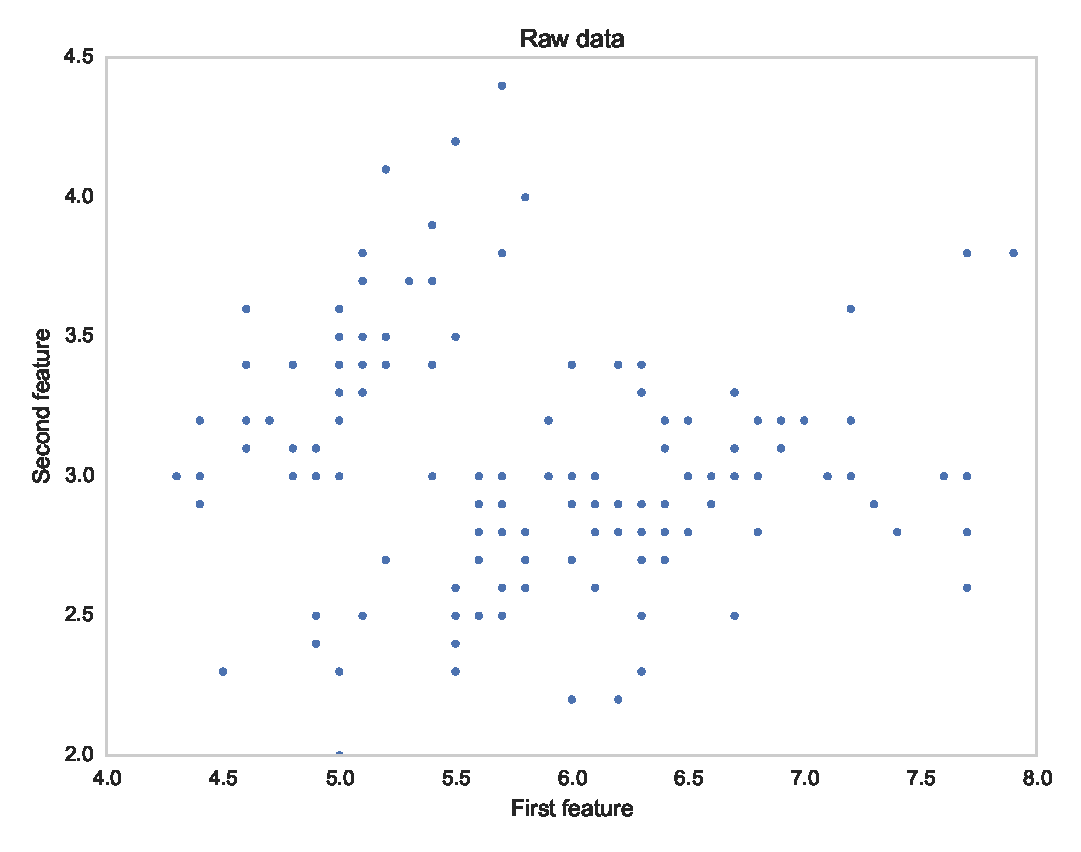
\includegraphics[width=\textwidth]{clustering/raw_data}
        \caption{Input data, unlabeled.}
        \label{fig:intro raw}
    \end{subfigure}
    %\hfill
    \begin{subfigure}[b]{0.45\textwidth}
        \centering
        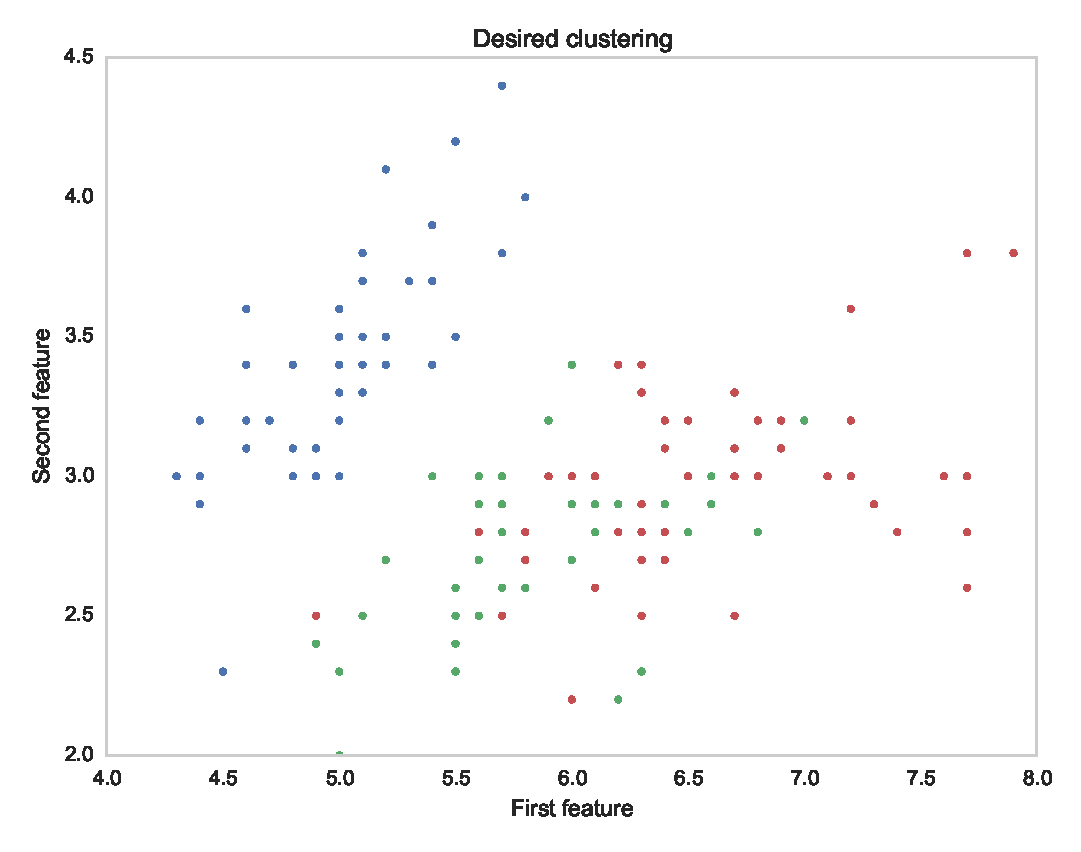
\includegraphics[width=\textwidth]{clustering/desired}
        \caption{Desired labels.}
        \label{fig:intro natural}
    \end{subfigure}

    \caption{First and second features of the Iris dataset. Fig. \ref{fig:intro raw} shows the raw input data, i.e. how the algorithms "see" the data. Fig. \ref{fig:intro natural} shows the desired labels for each point, where each color is coded to a class.}
    \label{fig:clustering plots}
\end{figure}


\section{Definitions and Notation}

This section will introduce relevant definitions and notation within the clustering context that will be used throughout the rest of this document.

% TODO: review this part of the vector notation, it's fishy right now
%pattern, features
A \emph{pattern} $\mathbf{x}$ is a single data item and, without loss of generalization, it consists of a set of $d$ \emph{features} $x_i$ that characterize that data item, $\mathbf{x} = (x_1, \ldots, x_d)$, where $d$ is referred to as the dimensionality of the pattern.
%pattern set
A \emph{pattern set} (or data set) $\mathcal{X}$ is then the collection of all $n$ patterns $\mathcal{X} = \{ \mathbf{x}_1, \ldots, \mathbf{x}_n \}$.
The number of features is usually the same for all patterns in a given pattern set.

%classes
In cluster analysis, the desired clustering, typically, is one that reflects the natural structure of the data, i.e. the original true clustering.
In other words, one wants to group the patterns that came from the same state of nature when they were generated, the same \emph{class}.
A class, then, can be viewed as a source of patterns and the effort of the clustering algorithm is to group patterns from the same source.
Throughout this work, these classes will also be referred to as the "natural" or "true" clusterings.
%labels
\emph{Hard} clustering (or partitional) techniques assign a class label $l_i$ to each pattern $\mathbf{x}_i$.
The whole set of labels of a pattern set $\mathcal{X}$ is given by $\mathcal{L} = {l_1, \ldots, l_n}$.
%partition
% Throughout this document, the whole set of labels may also be referred to as a partition.
Closely related to the whole set of labels is the concept of a \emph{partition}, which completely describes a clustering in a different way.
A partition $P$ is a collection of $k$ \emph{clusters}.
A cluster $C$ is a subset of $nc$ patterns $\mathbf{x}_i$ taken from the pattern set, where the patterns belonging to one subset don't belong to any other in the same partition.
A clustering \emph{ensemble} $\mathbb{P}$ is a set of partitions from a given pattern set.
The relationship between the above concepts is condensed in the following expressions:

\begin{align}
    \mathbb{P} &= \left \{   P^1, P^2, \ldots P^N   \right \}  \label{eq:ensemble} \\
    P^j &= \left \{   C^j_1, C^j_2, \ldots C^{j}_{k_j}   \right \}  \label{eq:partition} \\
    C^j_i &= \left \{   x_1, x_2, \ldots x_{nc^j_i}   \right \} \label{eq:cluster}
\end{align}


%similarity
Finally, a \emph{similarity measure} is a way of quantifying how similar two patterns are in the feature space, e.g. a metric (such as the euclidean distance), Pearson correlation.%TODO reference for a method for both euclidean distance and Pearson correlation

\section{Characteristics of clustering techniques}

Clustering algorithms may be described according to different properties.
For the sake of completeness, a small discussion of some properties will be layed out in this section.

% hierarchical and partitional
\emph{Partitional} and \emph{hierarchical} algorithms are the two most studied kinds of algorithms \cite{Aggarwal2014}.
A partitional algorithm is an hard clustering algorithm that will output a partiton where each pattern belongs exclusively to one cluster, e.g. K-Means.
A hierarchical algorithm produces a tree-based data structure called \emph{dendrogram}.
A dendrogram contains different partitions at different levels which means that the user can easily change the desired number of clusters by simply traversing the different levels.
This is an advantage over a partitional algorithm since a user can analyze different partitions with different numbers of clusters without having to rerun the algorithm.
% agglomerative vs divisive
Hierarchical algorithms can be further split into two approaches: bottom-up (or \emph{agglomerative}) and top-down (or \emph{divisive}).
% agglomerative
The former starts with all patterns as distinct clusters and will group them together according to some similarity measure, building the dendrogram from the ground up, e.g. Single-Link, Average-Link.
%divisive
The later will start will all patterns in the same cluster and continuosly split it until all patterns are separated, building the dendrogram from the top level to the bottom, e.g. Principal Directon Divisive Partitioning\cite{Boley1998} and Bisecting K-Means \cite{Steinbach2000}.


% monothetic vs polithetic
Another characteristic relates to how algorithms use the features for computing similarities.
If all features are used simultaniously the algorithm is called \emph{polithetic}, e.g. K-Means.
Otherwise, if the features are used sequentially, it's called \emph{monothetic}, e.g. \cite{Chavent1998}.

% fuzzy clustering
Constrasting \emph{hard} clustering algorithm are the \emph{fuzzy} algorithms.
A fuzzy algorithm will attribute to each pattern a degree of membership to each cluster.
A partition can still be extracted from this output by choosing, for each pattern, the cluster with higher degree of membership.
An example of a fuzzy algorithm is the Fuzzy C-Means \cite{Bezdek1984}.

% stochastic vs deterministic
Another characteristic is an algorithm's stochasticity.
A \emph{stochastic} algorithm uses a random search over the feature space at some point in its execution, possibly yielding different results in each run, e.g. K-Means can use a random initialization.
A \emph{deterministic} algorithm, on the other hand, will always produce the same result for a given input, e.g. Single-Link.

Finally, the last characteristic discussed is how an algorithm processes the input data.
An algorithm is said to be \emph{incremental} if it processes the input incrementally, i.e. taking part of the data, processing it and then doing the save for the remaining parts, e.g. PEGASUS \cite{Kang2011}.
A \emph{non-incremental} algorithm, on the other hand, will process the whole input in each run, e.g. K-Means.
This discussion is specially relevant when considering large datasets that may not fit in memory or whose processing would take too long for a single run and is therefore done in parallel.



% % examples of cluster analysis
% Cluster analysis is a relevant technique across several domains (\cite{Aggarwal2014}):

% \begin{itemize}
% 	\item grouping users with similar behaviour or preferences in \textbf{customer segmentation};
% 	\item image segmentation in the field of \textbf{image processing};
% 	\item clustering gene expression data, among other application, in the domain of \textbf{biological data analysis};
% 	\item generation of hierarchical structure for easy access and retrieval of \textbf{information systems}; % not referenced in book
% \end{itemize}

% Clustering is used in a wide variety of fields to solve numerous problems, e.g.:
% %TODO provide references to all of this
% % see https://sites.google.com/site/dataclusteringalgorithms/clustering-algorithm-applications
% % has applications with articles
% \begin{itemize}
% \item image segmentation in the field of image processing;
% \item generation of hierarchical structure for easy access and retrieval of information systems;
% \item recommender systems by grouping users by their behaviour and/or preferences;
% \item clustering customers for targeted marketing in 
% \item clustering gene expression data in biology;
% \item grouping of 
% \end{itemize}



\section{K-Means}

One of the most famous non-optimal solutions for the problem partitional clustering is the K-Means algorithm \cite{kmeansoriginal}.
The K-Means algorithm uses $K$ \emph{centroid} representatives $c_k$ for $K$ clusters.
Patterns are assigned to a cluster such that the squared error (or, more accurately, squared similarity measure) between the cluster representatives and the patterns is minimized.
In essence, K-Means is a solution (although not necessarily an optimal one) to a optimization problem having the Sum of Squared Errors as its objective function, which is known to be a computationally NP hard problem \cite{Jain2010}.
It can be mathematically demonstrated that the optimal representatives for the clusters are the means of the patterns of each cluster \cite{Aggarwal2014}.
K-Means, then, minimizes the following expression, where the similarity measure used is the Euclidean distance:

\begin{align}
    \sum^K_{k=1} \sum_{\mathbf{x}_i \in C_k} \| \mathbf{x}_i - c_k  \| ^2  \label{eq:sse}
\end{align}

K-Means needs two initialization parameters: the number of clusters and the centroid initializations.
It starts by assigning each pattern to its closer cluster based on the cluster's centroid.
This is called the \textbf{labeling} step since one usually uses cluster labels for this assignment.
The centroids are then recomputed based on this assignment, in the \textbf{update} step.
The new centroids are the mean of all the patterns belonging to the clusters, hence the name of the algorithm.
% convergence
These two steps are executed iteratively until a stopping condition is met, usually the number of iterations, a convergence criteria or both.
The initial centroids are usually randomly chosen, but other schemes exist to improve the overall accuracy of the algorithm, e.g. K-Means++ \cite{Arthur2007}.
There are also methods to automatically choose the number of clusters \cite{Aggarwal2014}.

% similarity measures
The similarity measure used is typically the Euclidean distance.
This tends to produce hyperspherical clusters \cite{Jain1999}.
Still, according to \cite{Jain2010}, other measures have been used such as the L1 norm, Mahalanobis distance, as well as cosine similarity \cite{Aggarwal2014}.
The choice of similarity measure must be made carefully as it may not guarantee that the algorithm will converge.

% empty clusters
A detail of implementation is what to do with clusters that have no patterns assigned to them.
One approach to this situation is to drop the empty clusters in further iterations.
However, allowing the existence of empty clusters or dropping empty clusters is undesirable since the number of clusters is an input parameter and it's expected that the output contains the specified number of clusters.
Other approaches exist dealing with this problem, such as equaling the centroid of an empty cluster to the pattern furthest away from its assigned centroid or reusing the old centroids as in \cite{Pakhira2009}.

% kmeans as a step for other algorithms
K-Means is a simple algorithm with reduced complexity $O(ntk)$, where $k$ is the number of clusters and $t$ is the number of iterations that it executes.
Because of this, K-Means is often used as foundational step of more complex and robust algorithms, such as EAC.

% After the first iteration, the first step is executed with the new centroids.
% The end result of the algorithm is the labels produced in the first step of the last iteration.

% The sequential K-Means algorithm is composed by two main stages \cite{Jain2010}:

% \begin{enumerate}
%     \item \textbf{labeling stage} for the assigning labels to each pattern of the data set, e.g. the label of the $i-th$ pattern is $0$ if the minimum distance is to the $0-th$ centroid;
%     \item \textbf{update stage} for the computation of the new centroids based on the labels assignment, i.e. the new centroids will be the mean of all the patterns assigned to it.
% \end{enumerate}

%example
As an example, the output of the K-means algorithm to the data presented in Fig. \ref{fig:clustering plots} is represented in Fig. \ref{fig:intro kmeans}.
The algorithm executed with 3 random centroids.

\begin{figure}[hbtp]
    \centering
    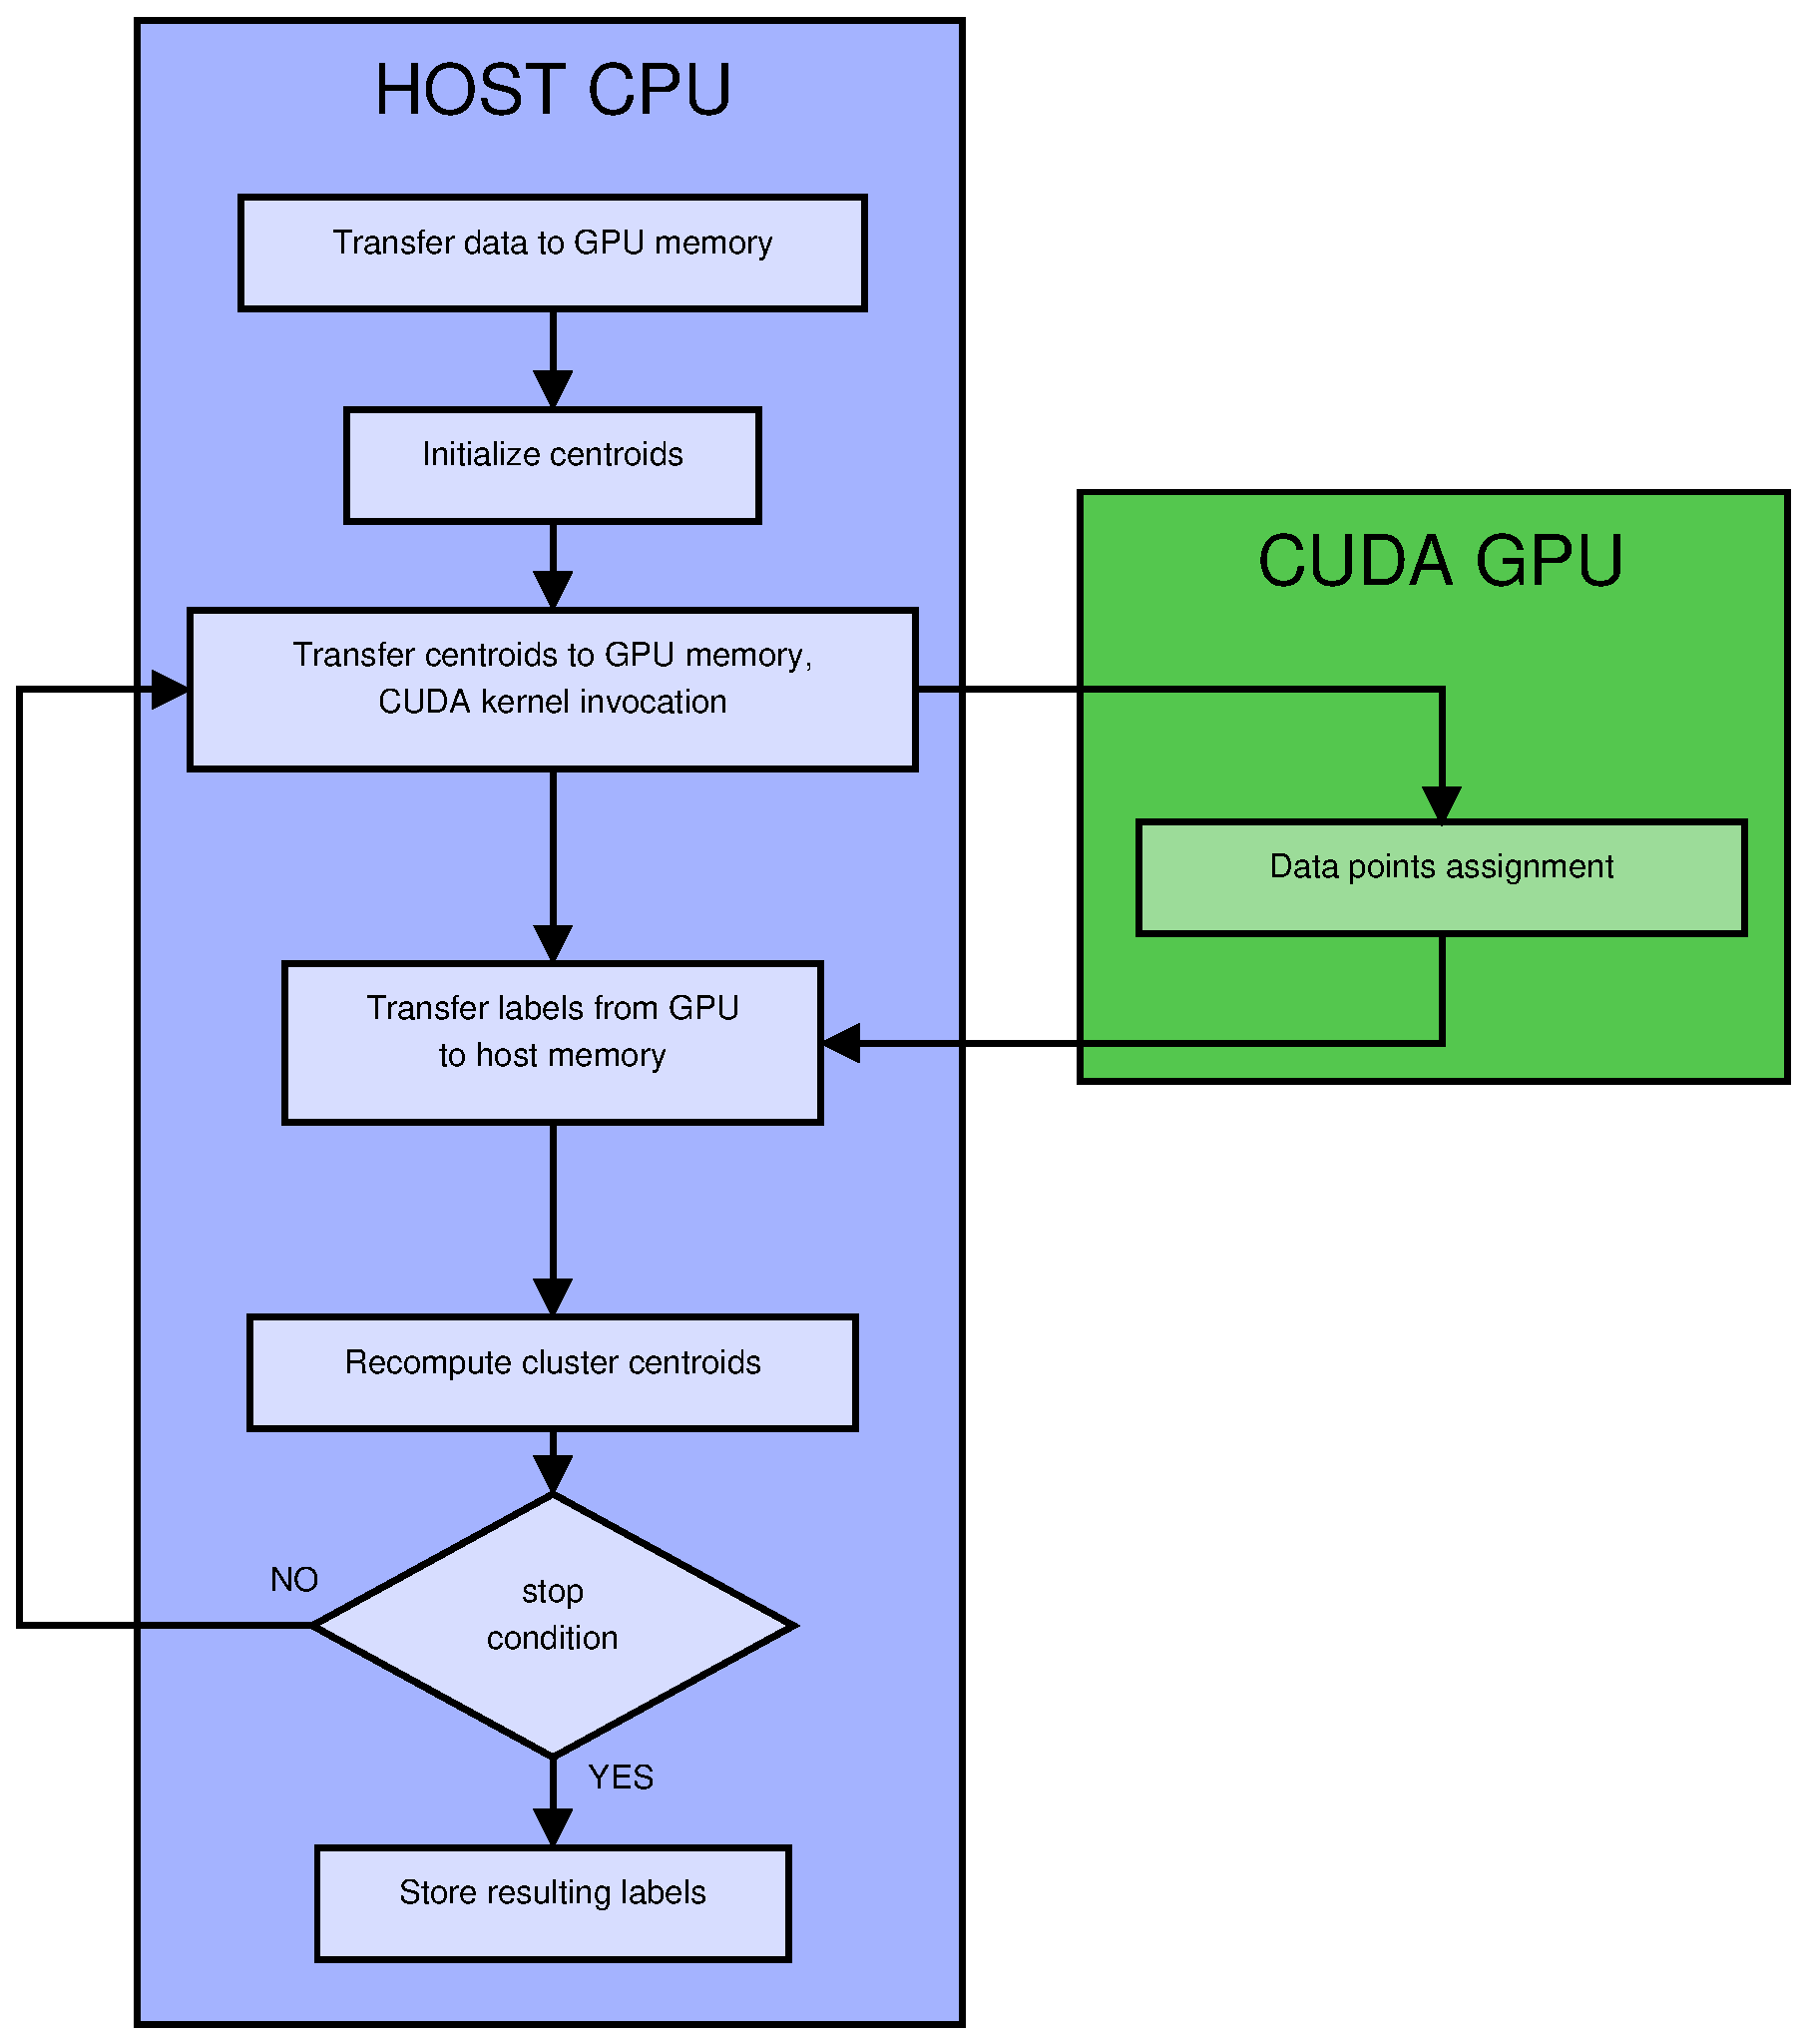
\includegraphics[width=0.5\textwidth]{clustering/kmeans}
    \caption{The output labels of the K-Means algorithm with the number of clusters (input parameter) set to 3.}
    \label{fig:intro kmeans}
\end{figure}

Even with the correct number of clusters, the clustering results don't match $100\%$ the natural clusters.
The accuracy relative to the natural clusters of Fig. \ref{fig:intro natural} is $88\%$ as measured by the Consistency Index (CI) \cite{Fred2001}.
In this example, the problem is the two overlapping clusters.
It's hard for an algorithm to discriminate between two clusters when they have similar patterns.
When no prior information about the dataset is given, the number of clusters can be hard to discover.
This is why, when available, a domain expert may provide valuable insight on tuning the initialization parameters.

\section{Single-Link}

Single-Link \cite{sneath1962numerical} is one of the most popular agglomerative hierarchical clustering algorithms.
It operates over a pair-wise similarity matrix and outputs a dendrogram (e.g. Fig \ref{fig:sl dendrogram}).
It starts by considering that every pattern is a cluster singleton.
In each iteration, the two most similar clusters are merged.
The similarity between two clusters is the similarity between their most similar patterns.
Because the algorithm connects first clusters that are more similar, it naturally gives more importance to regions of higher density \cite{Aggarwal2014}.
The algorithm stops when $n-1$ merges have been performed, which is when all patterns have been connected in the same cluster.
Just like in the K-Means algorithm, different similarity measures can be used for the distances.

A naive implementation of Single-Link comprehends the following steps \cite{Jain1999}:
\begin{enumerate}
    \item Create a pair-wise similarity matrix of all patterns, where each  pattern is a distinct cluster;

    \item Find the most similar clusters, merge them and uptade the matrix to reflect this change. The rows and columns of the two merged clusters are deleted and a new row and column are created to store the new cluster whose similarities to other clusters will be the minimum of either the merging clusters.

    \item Stop if all patterns belong to a single cluster, otherwise continue to step 2.
\end{enumerate}

% naive & SLINK
The total time complexity of this naive implementation is $O(n^3)$ since it performs a $O(n^2)$ search in step two and it does it $n-1$ times.
Over time, more efficient implementations have been proposed, such as SLINK \cite{Sibson1973}.
SLINK needs no working copy of $O(n^2)$ the pair-wise similarity matrix (if the original can be modified), has a working memory of $O(n^2)$ and time complexity of $O(n^2)$.
This increase in performance comes from the observation that the $O(n^2)$ search can be transformed in a $O(n)$ search at the expense of keeping two arrays of length $n$ that will store the most similar cluster for each pattern and the corresponding similarity measure.
This way, to find the two closest clusters, the algorithm will not search the entire similarity matrix, but only the new similarity array since this array keeps the closest cluster of each cluster.
Naturally these arrays must be updated upon a cluster merge.

% SL from MST
An interesting property of the Single-Link algorithm is its equivalence with a Minimum Spanning Tree (MST), an observation first made by \cite{Gower1969}.
In graph theory, a MST is a tree that connects all vertices together while minimizing the sum of all the distance between them.
An example of a graph and its corresponding MST can be seen in Fig. \ref{fig:mst example}.
In this context, the edges of the MST are the similarities between the patterns and the vertices are the patterns themselves.
A MST contains all the information necessary to build a Single-Link dendrogram.
To walk down through the levels of the dendrogram from the MST, one cuts the least similar edges.
Furthermore, this approach can be used to apply Single-Link clustering to graphs-encoded problems in a straight-forward way.
Furthermore, the performance properties of this method are the same as SLINK 
\cite{Mullner2011}.

\begin{figure}[!ht]
    \centering
    \begin{subfigure}[b]{0.3\textwidth}
        \centering
        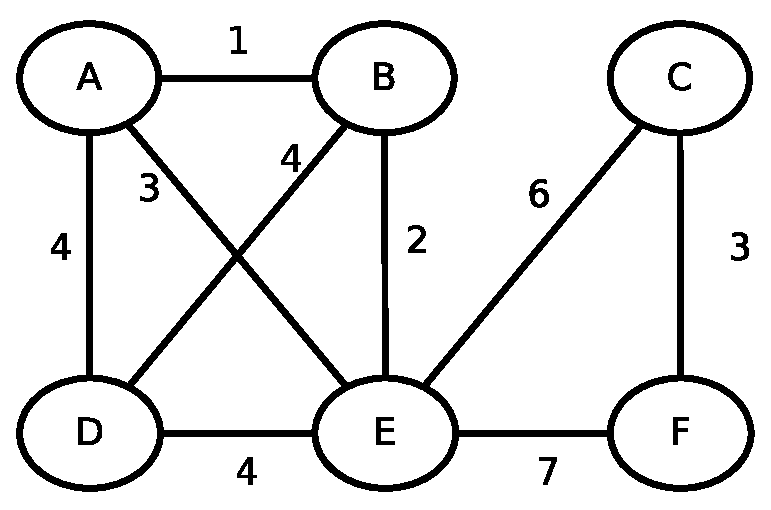
\includegraphics[width=\textwidth]{clustering/mst_graph}
        \caption{Example of a graph.}
        \label{fig:graph}
    \end{subfigure}
    %\hfill
    \hspace{30pt}
    \begin{subfigure}[b]{0.3\textwidth}
        \centering
        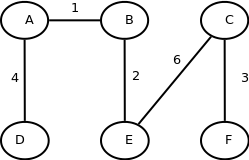
\includegraphics[width=\textwidth]{clustering/mst_mst}
        \caption{MST of graph to the left.}
        \label{fig:graph mst}
    \end{subfigure}

    \caption{The above figures show an example of a graph (left) and its corresponding Minimum Spanning Tree (right). The circles are vertices and the edges are the lines linking the vertices.}
    \label{fig:mst example}
\end{figure}

An example of a Single-Link dendrogram and resulting cluster can be observed in Fig. \ref{fig:sl plots}.
The dendrogram in Fig. \ref{fig:sl dendrogram} has been truncated to 25 clusters in the bottom level for the sake of readability.
The clustering presented on Fig. \ref{fig:sl clustering} is the result of cutting the dendrogram such that only 3 clusters exist (the number of classes).
The accuracy, as measured by the CI, is of $58\%$.

\begin{figure}[!ht]
    \centering
    \begin{subfigure}[b]{0.45\textwidth}
        \centering
        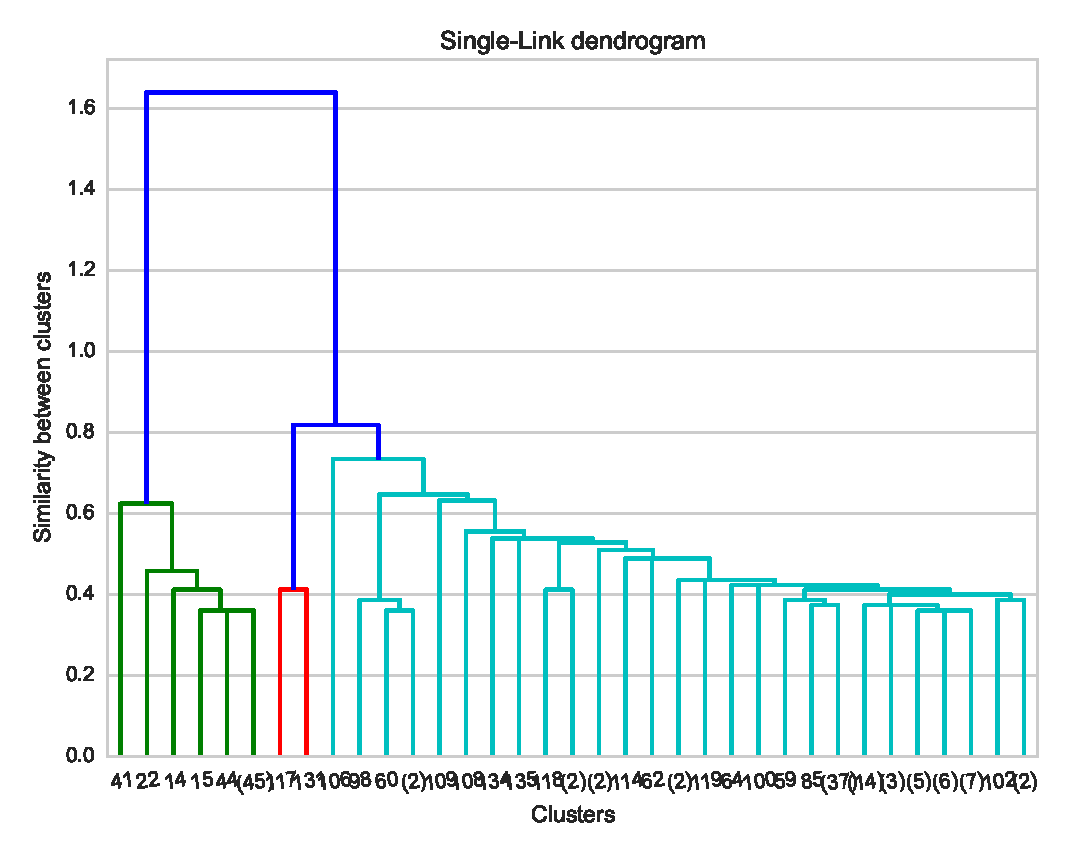
\includegraphics[width=\textwidth]{clustering/sl_dendrogram}
        \caption{Single-Link dendrogram truncated to 25 clusters in the bottom level.}
        \label{fig:sl dendrogram}
    \end{subfigure}
    %\hfill
    \begin{subfigure}[b]{0.45\textwidth}
        \centering
        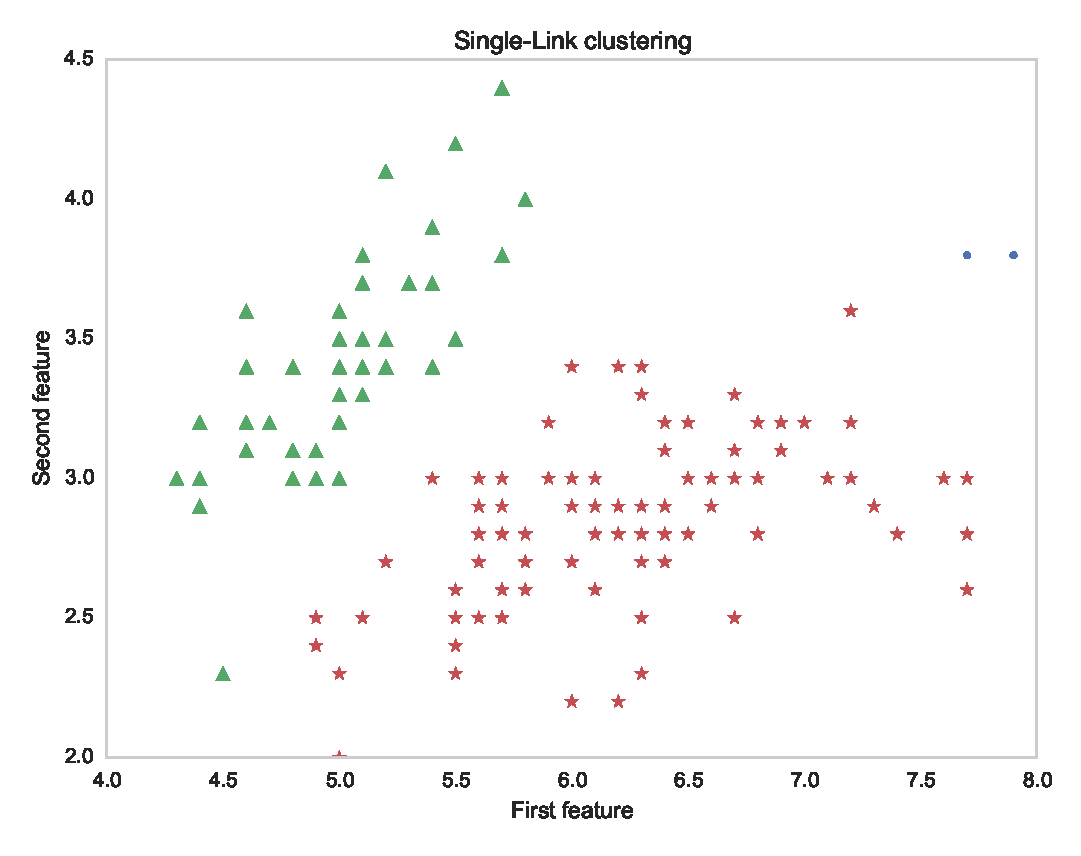
\includegraphics[width=\textwidth]{clustering/sl}
        \caption{Clustering with 3 clusters.}
        \label{fig:sl clustering}
    \end{subfigure}

    \caption{The above plots show the dendrogram and a possible clustering taken from a Single-Link run over the Iris data set. Fig. \ref{fig:sl clustering} was obtained by performing a cut on a level that would yield a partition of 3 clusters.}
    \label{fig:sl plots}
\end{figure}